\chapter{Overview of the Single-Phase Detector Module Design}
\label{ch:fdsp-ov}

%%%%%%%%%%%%%%%%%%%%%%%%%%%%%%%%%%%%%%%%%%%%%%%%%%%%%%%%%%%%%%%%%%%%
\section{Description}
\label{sec:fdsp-ov-model}

The DUNE-SP module features 10~kTon active mass LArTPC, with all associated cryogenic, electronic readout, computing, and safety systems.  The detector is designed to maximize the active volume within the confines of the membrane cryostat while minimizing dead regions.  The detector elements have been modularized such that their production can proceed in parallel with the construction of the DUNE caverns and cryostats, and sized so that they conform to the access restrictions for transport underground.  Table \ref{tab:dune-sp-parameters} summarizes some of the high-level parameters of the DUNE-SP detector.

\begin{dunetable}[DUNE-SP Parameters]{lll}{tab:dune-sp-parameters}{DUNE-SP Parameters}
Parameter & Value & Note \\ \toprowrule
Cryostat LAr Mass & 17.5~kTon & \\
Active LAr Mass & 10~kTon & \\ 
Active Height & 12~m & \\ 
Active Length & 57.5~m & \\ 
Maximum Drift & 3.6~m & \\ \colhline 
%Number of APAs & 150 & \\ 
%Number of CPAs & XXX & \\ 
%Number of PDs & XXX & \\ \colhline
Number of APA Channels & 384,000 & \\
Number of PDS Channels & 1500 & \\ \colhline
\end{dunetable}

\fixme{Fix all numbers in previous table.}

The cryostat will be constructed such that its long axis is aligned with the beam arriving from Fermilab.  The TPC detector inside the cryostat is composed of two rows of Cathode Plane Arrays (CPAs) oriented along the long axis of the cryostat, flanked on either side by rows of Anode Plane Assemblies (APAs).  A field cage (FC) completely surrounds the four
open sides of the four drift regions to ensure that the electric field within is uniform and unaffected by the presence of the cryostat walls and other nearby conductive structures.  Integrated within each APA are elements of the Photon Detection System (PDS) as well as electronics to process the APA signals.  Around the periphery of the TPC various instrumentation for monitoring the cryogenic environment is present.  Outside of the cryostat, additional electronic readout and data acquisition equipment is present to transfer information from the detector.  Figure~\ref{fig:dune-sp-overview} illustrates the basic arrangement of the TPC elements within the DUNE-SP detector.

\begin{dunefigure}[DUNE Single-Phase Far Detector Diagram]{fig:dune-sp-overview}{A diagram showing the arrangement of the main TPC elements in the DUNE-SP detector.  Two rows of CPAs are interleaved with three rows of APAs.  The FC structure (only partially depicted to enable visibility of other elements) surround the outer area of the APA and CPA rows.  Elements of the PDS are integrated within the APA structure.}
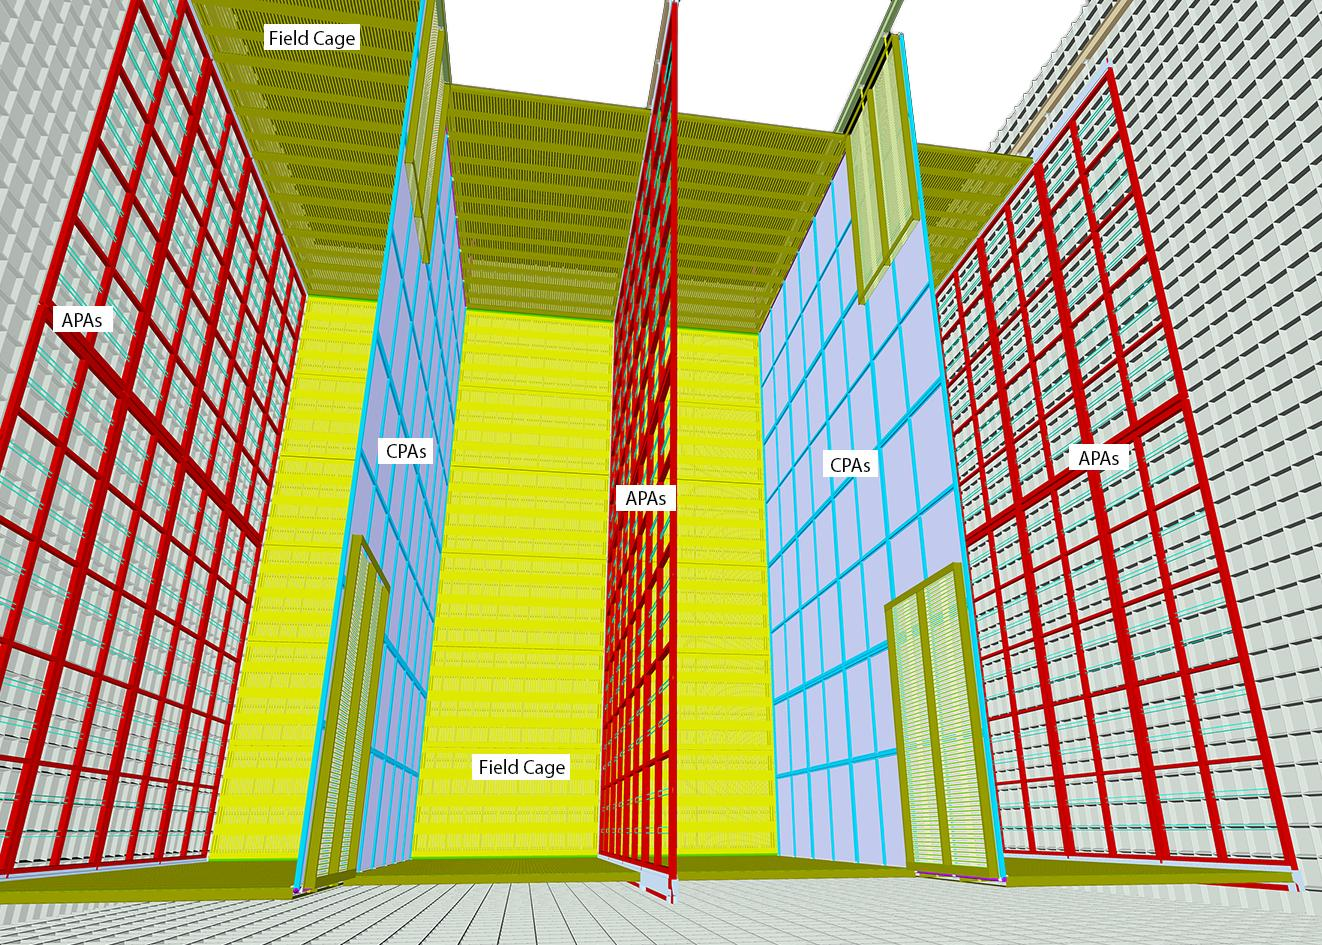
\includegraphics[width=0.6\linewidth]{DUNE-SP.jpg}
\end{dunefigure}



%%%%%%%%%%%%%%%%%%%%%%%%%%%%%%%%%%%%%%%%%%%%%%%%%%%%%%%%%%%%%%%%%%%%
\section{Primary Detector Systems}
\label{sec:fdsp-ov-sys}


%The elements composing the DUNE-SP detector module include the time projection chamber (TPC), the cold electronics (CE), and the photon detection system (PDS).  The TPC components, e.g., anode planes, cathode planes and the field cage, are designed in a modular way.  
%The six APAs are arranged into two APA planes, each consisting of three side-by-side APAs. Between them,  
%a central cathode plane, composed of 18 CPA modules, splits the TPC volume into two electron-drift regions, one on each side of the cathode plane. 
 
%\begin{itemize}
%\item{APA - Anode Plane Assemblies.}
%\item{HV - High Voltage system.  This system is composed of the Cathode Plane Arrays (CPAs), Field Cage (FC), and HV feedthrough.}
%\item{Electronics}
%\item{PD - Photon Detection System}
%\item{DAQ - Data Acquisition System}
%\item{CISC - Cryogenic Instrumentation and Slow Controls}
%\end{itemize}


Table~\ref{tab:tpc-systems} lists the principal detection systems of the DUNE-SP detector module along with the primary purpose of each system.  In this section, the primary detector systems are introduced briefly.  The subsequent chapters of this document provide extensive description of each of these systems. 

\begin{dunetable}[Single-Phase Far Detector Systems]{lll}{tab:tpc-systems}{Single-Phase Far Detector Systems.}
System & Name  & Purpose   \\  \toprowrule
\hyperref[ch:fdsp-apa]{APA}  & Anode Plane Assemblies & Ionization signal development \\
\hyperref[ch:fdsp-hv]{HV} & High Voltage & Establish uniform drift field \\
\hyperref[ch:fdsp-tpc-elec]{Elec} & Electronics & Process APA signals  \\
\hyperref[ch:fdsp-pd]{PD} & Photon Detection & Light collection and triggering\\
\hyperref[ch:fdsp-daq]{DAQ} & Data Acquisition & Record/handle digital data \\
\hyperref[ch:fdsp-slow-cryo]{CISC} & Cryogenic Instrumentation and Slow Controls & Maintain and monitor LAr volume\\ 
\end{dunetable}

%\begin{dunetable}[Single-Phase Far Detector TPC components, dimensions and
%    quantities]{lll}{tab:tpc-components}{Single-Phase Far Detector TPC components, dimensions and quantities}
%Detection Element & Approx Dimensions  & Quantity   \\  \toprowrule
%\hyperref{ch:fdsp-apa}{APA}  & 6~m H by 2.4~m W  & 50  per anode plane, 150 total  \\  \colhline
%CPA module  & 2~m H by 1.2~m W  & 6 per CPA column,   \\  
%  &  & 300 total  \\  \colhline
% Top FC module & 2.4~m W by 3.6~m along drift & XXX per top FC assembly, XXX total   \\  \colhline
% Bottom FC module & 2.4~m W by 3.6~m along drift & XXX per bottom FC assembly, XXX total   \\  \colhline
%End-wall FC module & 1.5~m H by 3.6~m along drift & XXX per end-wall assembly (vertical   \\  
%&  & drift volume edge), 16 total   \\  \colhline
%PD module  & 2.2 m $\times$ 86 mm $\times$ 6 mm & 10 per APA, 1500 total  \\ 
%\end{dunetable}


%%%%%%%%%%%%%%%%%%%%%%%%%%%%%%%%%%
\subsection{Anode Plane Assemblies}
\label{sec:fdsp-ov-apa}

The APA system, described in full detail in Chapter \ref{ch:fdsp-apa}, is used to capture the signals created by ionization drifting in the TPC volume.  Each APA features a metal frame, on each side of which there are three instrumented and two uninstrumented anode layers.  The design of the anode layers is arranged to provide three complimentary views of the ionization present in the TPC that can be combined to form three-dimensional representations of the distribution of the charge in the detector.  

Among the novel features of the DUNE-SP LArTPC are the presence of ``wrapped'' anode wires that follow a helical trajectory around the height of the APA.  This design choice was made to minimize the need to tile electronic readout around the perimeter of the APA, which would lead to dead space between neighboring APAs.  This choice also was driven by reconstruction performance, with the angle of the wrap chosen such that a given Induction plane wire does not intersect a given Collection plane wire more than once, which greatly reduces pathologies in pattern recognition. 


%%%%%%%%%%%%%%%%%%%%%%%%%%%%%%%%%%
\subsection{High Voltage}
\label{sec:fdsp-ov-hv}

The HV system, described in full detail in Chapter \ref{ch:fdsp-hv}, creates the uniform electric field in the TPC volume that causes ionization to drift towards the APAs.  The HV system contains both the CPAs, which are operated at a voltage of -180 kV, as well as the FC elements which progressively step the CPA voltage down in magnitude.  

Among the novel features of the DUNE-SP LArTPC is the use of resistive panels for the CPAs, which serves to control the flow of stored energy in the HV system in the event of an unexpected electrical discharge.  This features provides protection to the detector elements and guards against damage that would negatively impact detector performance.  



%%%%%%%%%%%%%%%%%%%%%%%%%%%%%%%%%%
\subsection{Electronics}
\label{sec:fdsp-ov-elec}

The electronics system, described in full detail in Chapter \ref{ch:fdsp-tpc-elec}, is responsible for manipulating the signals present on the APA wires and ultimately transferring them out of the cryostat and on to the DAQ system.  The first stage of low-noise electronics in the experiment are located directly on the end of the APA, where the ionization signals are initially shaped and amplified before further processing. 

\fixme{check how division between CE and readout is being addressed.}

%%%%%%%%%%%%%%%%%%%%%%%%%%%%%%%%%%
\subsection{Photon Detection}
\label{sec:fdsp-ov-pds}

The PD System, described in full detail in Chapter \ref{ch:fdsp-pd}, is used to capture scintillation light produced by interactions in the TPC.  The scintillation light of argon is very deep in the ultraviolet, so the PD elements are designed to shift this wavelength closer to the visible spectrum where the detectors have high efficiency.  

%%%%%%%%%%%%%%%%%%%%%%%%%%%%%%%%%%
\subsection{Data Acquisition}
\label{sec:fdsp-ov-daq}

The DAQ System, described in full detail in Chapter \ref{ch:fdsp-daq}, ...
%%%%%%%%%%%%%%%%%%%%%%%%%%%%%%%%%%
\subsection{Cryogenic Instrumentation and Slow Controls}
\label{sec:fdsp-ov-instr}

The CISC System, described in full detail in Chapter \ref{ch:fdsp-slow-cryo}, ...





